\chapter{Aplicación sobre datos}

\section{Cemento, análisis estructural y capacidades predictivas.}
\subsection*{Descripción del dataset}
\noindent El dataset  \cite{Yeh 2007} es un conjunto de datos recogidos de distintos tipos de cementos con distintas densidades, en particular tenemos las siguientes variables resumidas de manera esquemática en el cuadro \ref{tab:Resumen Variables}:
\begin{table}[h]
\footnotesize
\centering
\begin{tabular}{|l|l|l|l|}
\hline
Nombre & Tipo de dato & Medida & Descripción \\
\hline
Cemento (variable 1) & continuo & kg en una mezcla m3 & Variable predictora \\
Escoria de alto horno (variable 2) & continuo & kg en una mezcla m3 & Variable predictora \\
Ceniza volante (variable 3) & continuo & kg en una mezcla $m^3$ & Variable predictora \\
Agua (variable 4) & continuo & kg en una mezcla $m^3$ & Variable predictora \\
Superplastificante (variable 5) & continuo & kg en una mezcla $m^3$ & Variable predictora \\
Agregado grueso (variable 6) & continuo & kg en una mezcla $m^3$ & Variable predictora \\
Agregado fino (variable 7) & continuo & kg en una mezcla $m^3$ & Variable predictora \\
Edad & continuo & Día (1-365) & Variable predictora \\
Resistencia a la compresión & continuo & MPa & Variable respuesta \\
\hline
\end{tabular}
\caption{Resumen de las variables estudiadas}
\label{tab:Resumen Variables}
\end{table}




\noindent El tamaño de la muestra es de 1030 observaciones, de las cuales un $70\%$ se separan para realizar el ajuste de los distintos modelos y el $30\%$ restante se utilzará para calcular la capacidad predictiva de los modelos. 

\subsection*{Objetivos}

\noindent Este estudio tiene dos objetivos principales:
\begin{itemize}
\item Detallar y analizar patrones de comportamiento en los cementos en base a las características descritas. 
\item Crear y analizar distintos modelos que permitan la predicción de la resistencia a la compresión. 
\end{itemize}
\subsection*{Metodología}

\noindent Para conseguir el primer objetivo se utilizará el análisis de componentes principales. Con ello, se podrá estudiar la estructura de los datos de manera que se vea que variables afectan en mayor medida a la varianza. 

\noindent Para el otro objetivo se ajustarán   tres modelos distintos. Un modelo de regresión lineal, un árbol de regresión y una red neuronal. Se describirán las cualidades que aporta cada uno de los modelos y se compararán. Es por ello que se separará el conjunto de datos en dos partes una de ajuste y otra de comprobación de las capacidades predictivas. 

\noindent En particular, se utilizará el error cuadrático medio, \emph{MSE}, junto al coeficiente de determinación $R^2$ en cada uno de los modelos. 

\noindent A nivel técnico, para esta parte se utilizará el lenguaje de programación Python. En particular, se usan las siguientes librerías:
\begin{itemize}
\item \emph{Pandas:} para el tratamiento previo de los datos \cite{Pandas}. 
\item \emph{Scikit-Learn y Tensor-Flow:} usado en el ajuste de los distintos modelos \\ \cite{Scikit-Learn, TensorFlow}. 
\item \emph{NumPy:} utilizado en el manejo de las matrices y los vectores \cite{Numpy}. 
\item \emph{Matplotlib} empleado para la generación de los distintos gráficos \cite{Matplotlib}
\end{itemize}

\subsection*{Desarrollo y resultados}

\noindent Para empezar, se hace un análisis descriptivo básico de cada una de las variables:
\begin{figure}[h]
  \centering
  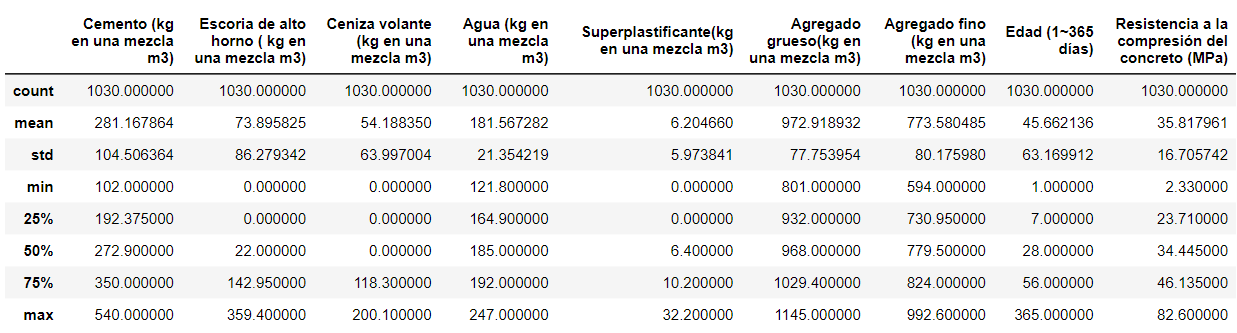
\includegraphics[scale=0.55]{Documentos Extra/Imagenes/Resumen_Basicos.png}
  \caption{Análisis descriptivo de los datos}
  \label{fig:resumen_basicos}
\end{figure}

\noindent En este primer análisis resumido en la figura \ref{fig:resumen_basicos} podemos ver que la media de la fuerza de compresión o resistencia a la compresión tiene una media muestral de $35,82$ MPa, con una desviación estándar de $16,70$ MPa lo cual nos dice que hay una alta dispersión de los datos en este caso. Hay que tenerlo en cuenta ya que puede provocar que no se den los resultados deseados. 

\noindent Hay otras medidas a las que le ocurre lo mismo, es decir, que tienen una alta dispersión como pueden ser las cantidad de superplastificante, la ceniza volante o la escoria de horno. 

\noindent También hay que destacar que al menos un $50\%$ de las observaciones no tiene ceniza volante.  

\noindent Ahora se calculan las componentes principales utilizando la matriz estandarizada. Después de aplicar este proceso, obtenemos la proporción de la varianza explicada en cada una de las componentes:
\begin{equation*}
(0.25 \enspace 0.22 \enspace 0.16 \enspace 0.12 \enspace 0.11 \enspace 0.09 \enspace 0.03 \enspace 0.02 \enspace 0.  )
\end{equation*}

\noindent En particular, son las primeras componentes las que mayor variabilidad explican, de esta manera que la 3 primeras acumulan más del $62\%$ de la varianza y si tomamos hasta tener 5 se llega casi a un $85\%$ de la variabilidad total de los datos. En nuestro caso, estudiaremos las cualidades de las 3 primeras, ya que en caso de necesitarse sería posible hacer una representación de los datos. 

\noindent Concretamente, los coeficientes de las 3 componentes principales son los siguientes :
\begin{align}
Z_1&=(0.04 \enspace 0.16  \enspace  -0.37  \enspace 0.56  \enspace   -0.54  \enspace  0.06 \enspace  -0.38  \enspace 0.26  \enspace -0.11)\mathbf{x}^T\\
Z_2&=(0.54 \enspace 0.14 \enspace  -0.27  \enspace -0.12 \enspace   0.25  \enspace -0.22 \enspace  -0.19 \enspace  0.25  \enspace  0.63)\mathbf{x}^T\\
Z_3&=(0.36 \enspace -0.7 \enspace  0.02 \enspace-0.12\enspace -0.19  \enspace 0.55 \enspace 0. \enspace   0.17 \enspace 0.03)\mathbf{x}^T
\end{align}

\noindent Al haber trabajado con la matriz estandarizada, estas cargas representan la correlación de cada una de las variables con la componente en cuestión. 

\noindent Aquellas variables que tienen una carga en las componentes principales mayor que $0.5$ en valor absoluto tienen una relación importante con las componentes. En cambio, todas aquellas cercanas al $0$ no tienen una relación significativa con la componentes. 

\noindent En el apartado de los modelos predictivos se han ajustado 3 modelos, para los cuales se han separado un $721$ muestras para entrenamiento y un $309$ para comprobación. Estas han sido elegidas para poder  
\noindent Las características de los modelos y de los procesos de ajuste son los siguientes:

\noindent El modelo lineal obtiene el siguiente modelo: \begin{equation}
Y=-51.45+0.13 X_1+0.11X_2+0.1X_3-0.12X_4+0.26X_5+  0.03X_6+0.03X_7+0.11X_8
\end{equation}
\noindent A destacar la mayor influencia en el modelo de la variable que mide la cantidad de superplastificante y la poca importancia en el modelo de tanto el agregado fino como el grueso, lo que implica que aumentar o disminuir la cantidad de dichos agregados no afectan a la resistencia a la compresión. En cambio añadir mayor cantidad de superplastificante aportará más a la fuerza de compresión.
  
\noindent A nivel predictivo, este modelo obtiene unos resultados en el conjunto de entrenamiento de un $MSE=108,35$ y un coeficiente de determinación $R^2=0.615$ lo cual nos indica que proporción de la variabilidad de la variable dependiente recoge el modelo. En cambio, el modelo en el caso del conjunto de pruebas obtiene un $MSE=106,02$ con un $R^2=0.61$. 

\noindent El caso del árbol de regresión, hay que destacar la diferencia que hay entre el error cuadrático medio en el conjunto de entrenamiento, $MSE=1,15$ mientras que el error cuadrático medio en el conjunto de prueba es de $MSE=53,28$. Por tanto, podemos estar ante un caso de sobre ajuste, en particular, en el caso del conjunto de entrenamiento el coeficiente $R^2=0.996$ y en el conjunto de prueba es $R^2=0.803$.  Por tanto, el modelo consigue reunir gran parte de la variabilidad de la variable respuesta. La siguiente figura \ref{fig:diagrama arbol} muestra la división que obtiene.
  

\noindent En el caso de la red neuronal se ha elegido un modelo con 2 capas una de entrada con 13 neuronas, en la cual se utiliza una función de activación lineal rectificada y una de salida con una neurona la cual utiliza la función identidad como función de activación. Con este modelo sencillo se consigue en el caso de los datos de entrenamiento, un $MSE=45,748$ y un coeficiente $R^2=0.837$. Por otro lado, en el conjunto de prueba se obtiene un error cuadrático medio de $MSE=51.805$ y un $R^2=0.809$.

\noindent En principio, el modelo más equilibrado sería el caso de la red neuronal, ya que no entra en sobre ajuste como el árbol de regresión ya que se ha obtenido una disparidad muy evidente del error en el conjunto de entrenamiento en comparación del error en el conjunto de prueba. Y el modelo de regresión lineal obtiene unos resultados malos. 

\begin{figure}[h]
  \centering
  \begin{minipage}{0.32\textwidth}
   
    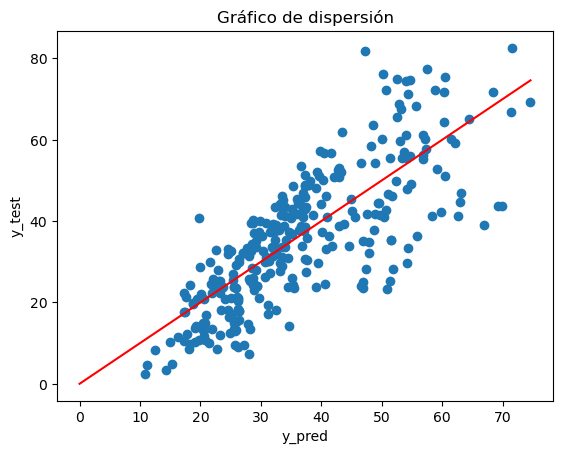
\includegraphics[width=\textwidth]{Documentos Extra/Imagenes/Datos PruebasRegresionLineal.png}
    \caption{Regresión Lineal}
    \label{fig:regresion_lineal}
  \end{minipage}
  \hfill
  \begin{minipage}{0.32\textwidth}
 
    \includegraphics[width=\textwidth]{Documentos Extra/Imagenes/Datos PruebasÁrbolesRegresion.png}
    \caption{Árbol de Regresión}
    \label{fig:regression_tree}
  \end{minipage}
  \begin{minipage}{0.32\textwidth}
    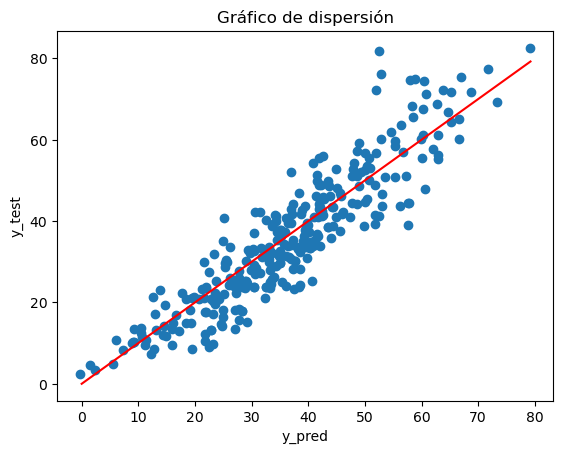
\includegraphics[width=\textwidth]{Documentos Extra/Imagenes/Datos PruebasRedNeuronal.png}
    \caption{Red Neuronal}
    \label{fig:red_neuronal}
  \end{minipage}
 \end{figure}





%\begin{table}[ht]
%\centering
%\begin{tabular}{|l|c|c|c|}
%\hline
% & Modelo Lineal & Árbol de Regresión &  Red Neuronal \\
%\hline
%Conjunto Ajuste &  $106.14$  &  $108.22$& $46.56$\\
%Conjunto de Prueba & $108,21$   & $57.55$ &  $47.54$ \\
%\hline
%\end{tabular}
%\caption{Errores cuadráticos medios en cada conjunto}
%\label{tab:tabla_ejemplo}
%\end{table}



